\section{Sandwich Debate}
\subsection{Sandwich Identification}
\begin{minipage}{.5\textwidth}
	\textbf{Sandwiches}
	\begin{itemize}
		\item BLT on white bread
		\item cheese quesadilla
		\item chip butty
		\item egg \& cheese biscuit
		\item grilled cheese
		\item hamburger
		\item ice cream sandwich
		\item patty melt
		\item sloppy joe
		\item tuna salad on brioche
		\item turkey and swiss on potato roll
		\item vada pav
		\item veggie burger
	\end{itemize}
\end{minipage}
\begin{minipage}{.5\textwidth}
	\textbf{Other}
	\begin{itemize}
		\item burrito
		\item buttered biscuit
		\item calzone
		\item chicken wrap
		\item gyro
		\item ice cream taco
		\item Klondike bar
		\item meatball sub
		\item sushi rolls
		\item toast
		\item toaster strudel
		\item turkey hero
	\end{itemize}
\end{minipage}


\subsection{Incremental Sandwich Learning}
\subsubsection{Initial Variabilization}
\begin{figure}[H]
	\centering
	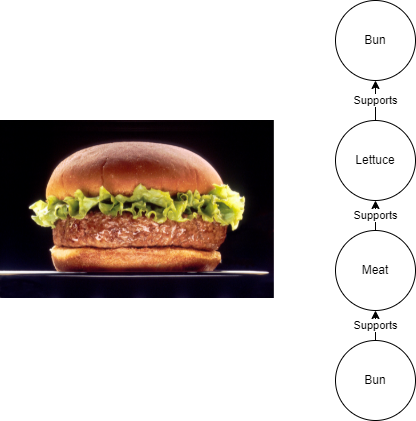
\includegraphics[height=6cm]{Figures/hamburger.png}
	\caption{Initial variabilization using the concept model of a hamburger--a positive example of a sandwich.}
	\label{fig:hamburger-concept}
\end{figure}
\subsubsection{Incremental Learning}
From the initial sandwich concept, the agent learns from a positive example of an ice cream sandwich, Figure \ref{fig:step1}.
\begin{figure}[H]
	\centering
	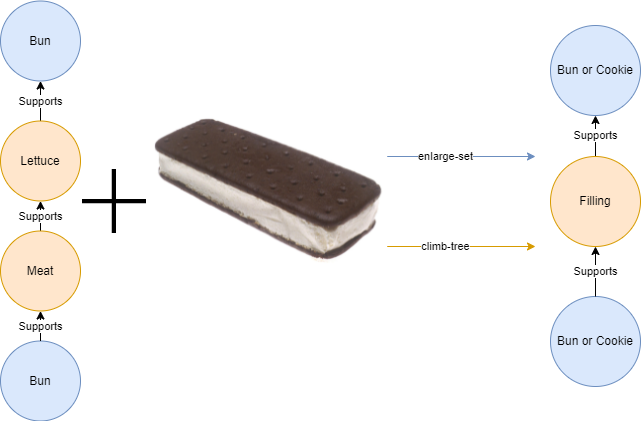
\includegraphics[height=6cm]{Figures/step1.png}
	\caption{Agent revising concept using a positive example of a sandwich. The agent would generalize using \textit{expand-set} to combine Bun and Cookie. Meat, Lettuce, \& Ice Cream may be abstracted to \textit{Filling}, though this would most likely require more background knowledge (see Appendix \ref{appendix:filling}) to use \textit{climb-tree}, or less detailed modeling. Concept model for Ice Cream Sandwich found in Appendix \ref{appendix:ics}}
	\label{fig:step1}
\end{figure}

\begin{figure}[H]
	\centering
	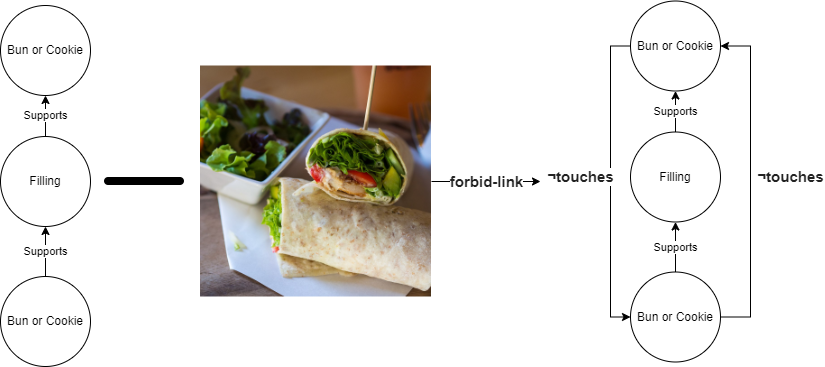
\includegraphics[height=6cm]{Figures/step2.png}
	\caption{Agent revising concept using a negative example. The agent would specialize using \textit{forbid-link} to represent that the two pieces of Bun or Cookie must not touch. Concept model for Chicken Wrap found in Appendix \ref{appendix:cw}}
	\label{fig:step2}
\end{figure}

\begin{figure}[H]
	\centering
	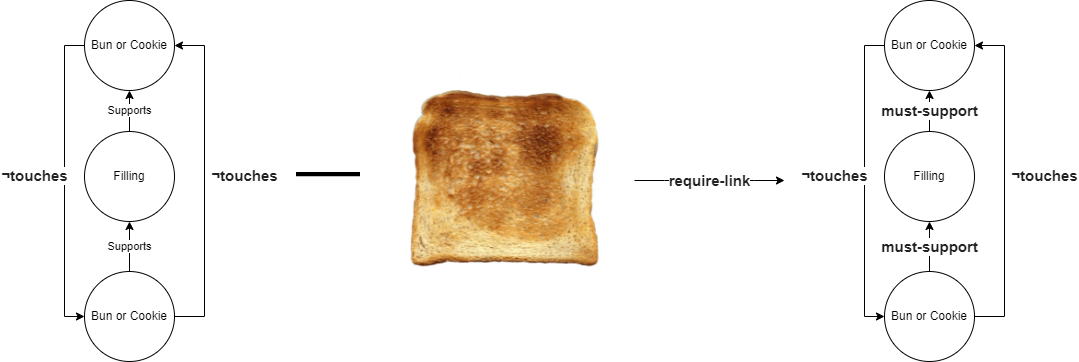
\includegraphics[height=6cm]{Figures/step3.png}
	\caption{Agent revising concept using a negative example. The agent would specialize using \textit{require-link} to represent that a piece of Bun or Cookie must-support the filling, and the Filling must-support a separate Bun or Cookie. Concept Model for Toast found in Appendix \ref{appendix:toast}}
	\label{fig:step3}
\end{figure}
\subsubsection{Honorable Mentions}
There are couple of other dishes that would have added significant changes to the concept model. One of these is the Klondike bar, which would most likely result in further specializing the surrounding shell of the dishes. That is, it would require that the outer two pieces of a sandwich be specifically of a grain type, or to not be chocolate. Additionally it would result in a require-link heuristic for the Filling , whereby it must-support a separate outer layer.

\subsection{Sandwich Classification}
\begin{table}[H] % [h] forces the table to be output where it is defined in the code (it suppresses floating)
	\caption{Classification Table for Sandwich}
	\small % Reduce font size
	\centering % Centre the table
	\begin{tabular}{L{0.17\linewidth} L{0.12\linewidth} L{0.12\linewidth} L{0.12\linewidth} L{0.12\linewidth} L{0.12\linewidth} L{0.12\linewidth}}
		\textbf{Attribute} & \textbf{Klondike Bar} & \textbf{Vada Pav} & \textbf{Buttered Biscuit} & \textbf{Calzone} & \textbf{Toast} & \textbf{Hamburger} \\
		\toprule[0.5pt]
		Made from layered ingredients? & Yes & Yes & Yes &	Yes &	No & Yes\\
		\midrule
		Has a filling? & Yes &Yes&	No&	Yes&	No&	Yes\\
		\midrule
		Outer layer made of grain? & No&	Yes&	No (partially)&	Yes&	Yes&	Yes\\
		\midrule
		Has contiguous outer layer? & Yes&	Yes	&No&	Yes&	Yes&No\\
		\midrule
		At least one side exposes filling? & No&	Yes&	N/A (No)&	No&	N/A (No) &	Yes \\
		\midrule
		Displayed on plate with filling plane parallel to plate? (visual in Appendix \ref{appendix:plate}) & N/A (No)&	Yes&	N/A (No)&	N/A (No)&	N/A (No)&	Yes
	\end{tabular}
\end{table}


\subsection{Sandwich Conclusion}
From the incremental learning model, a hotdog \textbf{would} be classified as sandwich. Although the hotdog lacks two distinct outer layers of grain, the concept model for a hotdog would resemble that of the Vada Pav sandwich. Specifically, it would have a single outer Grain layer supporting the filling. 

Utilizing Classification, a hotdog would \textbf{not} be classified as sandwich. This is due to the fact that a hotdog's \textit{intended} display results in the filling being orthogonal to the plate. Otherwise a hotdog covers each of the other attributes that would otherwise be required to be classified as sandwich.

From the perspective of case-based reasoning, the sandwich that would be most similar to a hotdog would most likely be the vada pav. From my understanding of this dish, it seems to resemble a hot-dog with the bun being sliced almost completely into halves, and some sort of filling placed inside. Unlike a hot-dog, I classify it as a sandwich due to the manner in which the vada pav is presented horizontally (see Appendix \ref{fig:vadapav}), resembling a burger slider. This may infer that case-based reasoning \textbf{would} identify a hotdog as a sandwich. 

In conclusion, I would claim that a hot-dog is a sandwich based on the arguments presented above. By way of majority voting, two out of the three techniques \textbf{would} identify a hotdog as a sandwich.
